This proposed project will be conducted over 24 months and will include three studies: (1) a descriptive analysis of retrospective data, (2) a laboratory based usability study, and (3) a randomized control trial.

 The first objective is needed to design both the control and experimental interventions and ensure they work with local data. Objective 2 will ensure that both interventions are usable and free from major bugs or obvious unintended effects. It will also be used to foresee any deployment issue with the hospital. Finally, objective 3 addresses the overall hypothesis, the effect of gamification on e-A\&F systems.

\begin{figure}[h]
    \centering
    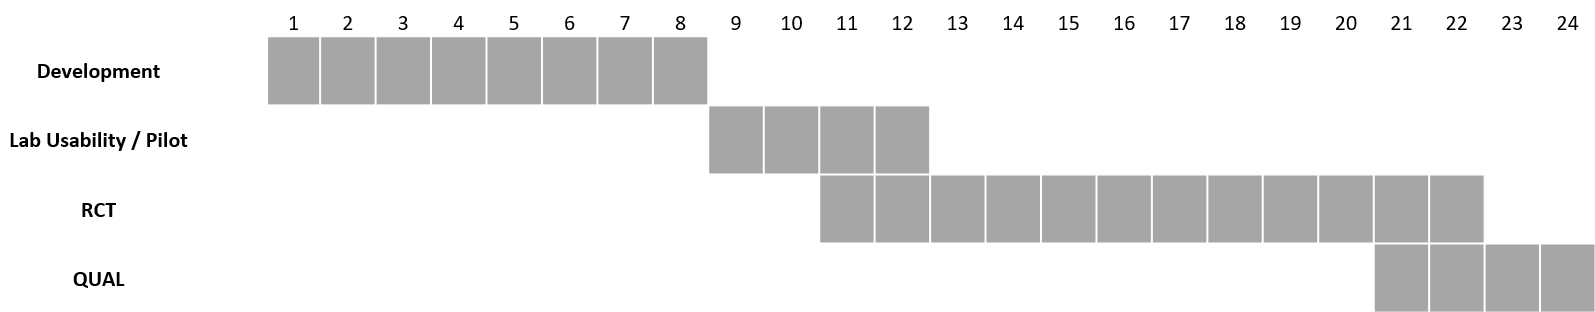
\includegraphics[width=\textwidth]{img/timeline-overall.PNG}
    \caption{Research Project, Timeline in months}
    \label{fig:timeline}
\end{figure}

\section{Data Source and Characteristics}

\begin{wrapfigure}{r}{10cm}
  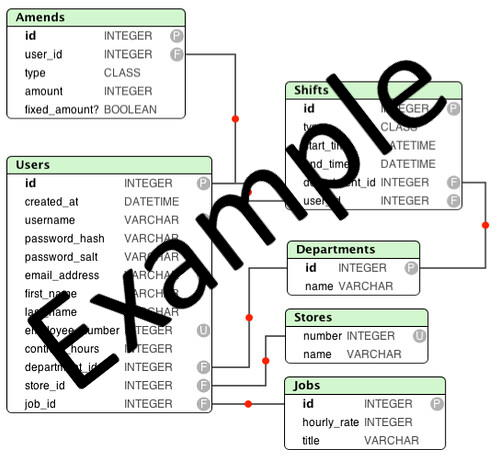
\includegraphics[width=\linewidth]{img/example_erd1.jpg}
  \caption{Entities and their relationship in the data}
  \label{fig:entity-relationship-diagram}
\end{wrapfigure}

The section discusses two distinct data needs. What is used for research and what is used in the interventions. The data for research is denominalized and seen by the research team, the data for the intervention is nominalized and only seen by the physician who undertook the care of the patient mentioned.

Patient and physician data will come from an existing system at the MUHC called the "data warehouse" (DW). A data warehouse is an enterprise data aggregation system which facilitates its collection, analysis, and reporting. The MUHC DW is already in place and contains a wide range of data relating to most aspects of in-hospital care.

This project will use two datasets coming from the same source. A first, broader and denominalized, data request will be made for the purpose of finding targets in objective one and two. This request will be placed to the research pipeline of the data warehouse. Here, the identity of both the patient or provider is of little interest as long as they have unique IDs. A second, precise, targeted, and nominalized data request will be made for the purpose of conducting the RCT. During this phase, I need to be able to have the right provider see the right feedback, but these providers also need to be able to see which patient might be in need of additional actions.

Additional data will be collected on the physician's use of e-A\&F. This data will be linked to anonymous IDs.

All nominalized data will be kept in a remote secure server in the MUHC data center. Feedback will also be created by the systems on this server. Anonymous data will be kept on a secure password protected computer, where the data analysis will also take place. All nominalized data will be removed as soon as the trial is over, while summary description of the anonymous data will be published along with the relevant research articles.

\chapter{Objective 1: Exploration of Metrics}
% Develop a set of quality indicators for e-A&F
Audit and feedback is first and foremost a way to generate new insights and inform future actions in clinical care. For this reason, the design and implementation of measurement is of critical importance to the creation of effective A\&F. The WHO describes performance measurement as a process which "seeks to monitor evaluate and communicate the extent to which various aspects of the health system meet their key objectives."\cite{smith2009performance} However, not all quality measures are created equal and the creation of suitable and successful metrics is not simple. Current evidence shows that quality measures should be aligned within an organizational context, relevant to its actors, attributable to specific individuals, feasible, accurate, and reliable.\cite{polanczyk2019quality}

For this reason, my first objective is to "develop a set of quality indicators for e-A\&F to assess and improve the appropriateness of heart failure management in adult patients at the MUHC." This set of indicators will then be used in objective 2 and 3 as it will impact (1) data collection, (2) feedback design, and (3) evaluation of the intervention.

\section{Research Design}
I propose an exploratory quantitative analysis of quality measures for heart failure at the MUHC. This study will use two years of retrospective secondary operational data to compare candidate quality measures. Data will be extracted by selecting admitted patients with ICD codes \footnote{From AHA's, Get with the Guidelines\textcopyright - Heart Failure} for heart failure along with the physicians who interacted with them. In order to match the future objective and limit the unnecessary risk to patients, data will be limited to adult patients at the MUHC.

\todo[inline]{Add information here on how many patients/doctors, we approximate this means based on Madjda numbers.}
\todo[inline]{How to justify 2 years (of HF patients, perc. complet in lit) }

Descriptive statistics will be used to provide a tabular overview of the stratified and unstratified measures, their completeness, along with a visual presentation of trends. The stratified exploration will explore the influence of basic patient demographic factors, of their cardiovascular risk, and of physician characteristics. 

\section{Evaluation Criteria}
\begin{itemize}
    \item Campbell's Prerequisites for quality measures (Acceptability, Feasibility, Reliability, Sensitivity, and Predictive Validity) \cite{campbell2002research}
    \item Key considerations when addressing causality and attribution bias (attribution, confounding, and risk adjustment) \cite{terris2009attribution}
    \item Characteristics of effective A\&F (baseline performance, availability of action plan, possible frequency, and latency)\cite{ivers2012audit} % i.e. (asap considering patient load)
\end{itemize}

Baseline performance, possible frequency, latency, attribution, and feasibility will be assessed using the basic statistics mentioned above. Acceptability will be taken into account in objective 2. Sensitivity to change, predictive validity, risk adjustment, and impact of confounders will be assessed using regression modeling. Availability of action plan will be checked manually with their relevant framework.

\section{Candidate Quality Indicators}
Multiple efforts have been made between institutions and advocacy groups to define a set of evidence-based actionable indicators for heart failure.\cite{hong2006overview}\cite{fonarow2010improving} \cite{kelley2006health} At this point, newer intervention are encouraged to use existing list of candidate measures instead of going to the source material. Doing so accelerate development and contributes to the soundness of the evidence, better face/content validity, reproducibility (between institutions), and more evidence on their association with significant health outcomes.\cite{smith2009performance}

The list of candidate retained is the result of a recently compiled systematic review of quality indicators in the ICU.\cite{goldfarb2018systematic} Its set of high-quality indicators will be considered first. But, if too few indicators are meeting the evaluation criteria, more indicator will be chosen from their expended list by local HF experts.

% Quality measures on heart failure can be from four domains: structure (), process (), outcome (), and patient experience (). The choice of quality measures has an important impact on A\&F since, for example, process measures are easier to collect and quicker to influence, but outcome measures are closer to the what healthcare is about. Measures which are stated or derived from more behavioural perspective seems to work better. Finally, quality measures which already have high compliance have, by the ceiling effect, less opportunity for improvement. 

\chapter{Objective 2: Pilot Assessment}
% Lab Usability testing
\begin{itemize}
    \item Basic Usability
    \item Topics of Comments
    \item Adverse Effects?
    \item Scalability and Deployment Testing/Planning
\end{itemize}

\chapter{Objective 3: Randomized Evaluation}
% Randomized Control Trial
https://library.gv.com/how-to-choose-the-right-ux-metrics-for-your-product-5f46359ab5be

\textbf{Randomized Control Trial with Qualitative Embedded Measure}

The proposed research design is a two-arm randomized control trial of a gamified e-A\&F system compared to an adapted existing system on the clinical performance of physicians in one hospital centre of Quebec. The control system will be adapted from an existing system’s user interface to include comparable information on users’ performance.

The project can be divided in three phases. In phase 1, the clinical team and research partners will work on the content of the A\&F intervention and at the same time an initial implementation of the system is performed. In phase 2, pilot testing is done in laboratory condition to study the system’s usability, the viability of the instruments, and assess the feasibility of the in-hospital deployment. Finally, phase 3 is a 12 months period in which clinicians are recruited, randomized, and data is collected on their practice and the use of the system. This phase will also contain a qualitative embedded study investigating the subject’s perceptions of different aspects of the A\&F system such as potential unintended effects or the adequacy of the targets.

The RCT 12 months is an trade off between longer time for ecologically relevant study period for sustained used and time feasibility concerns.
Some kind of impact evaluation could have been used, but an RCT will provide results which are likely to be more comparable with the literature, and therefore more easily usable 
\begin{figure}[h]
    \centering
    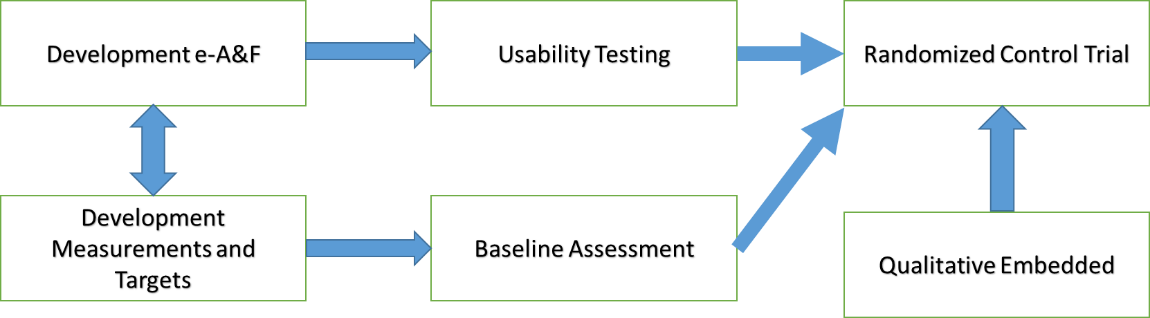
\includegraphics[width=\textwidth]{img/overall_sequence.png}
    \caption{Overall sequence, research project}
    \label{fig:ove_seq}
\end{figure}

The participants will be physicians and trainees from the participating department. Informed consent will be obtained and participants can step out at any time. Performance feedback will be confidential and personal. No clinical data will be captured specifically for this project, only secondary data will be used. The A\&F system will leverage the MUHC data warehouse to automate data collection.

\begin{figure}[h]
    \centering
    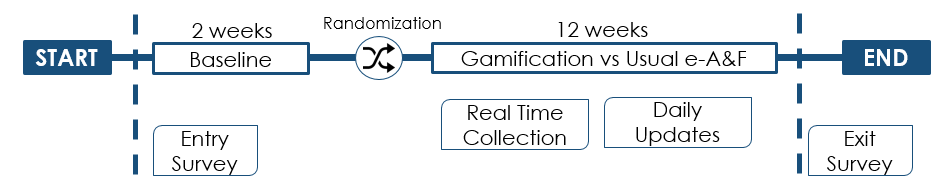
\includegraphics[width=\textwidth]{img/rct_flow.png}
    \caption{Diagram of the RCT process}
    \label{fig:rct_flow}
\end{figure}

\subsubsection{Participants}
* Attending Physicians, Residents (Cardiology, and others), Fellow

Physicians of the cardiology ward, at the MUHC Glen hospital.

Includes : Attending physicians, residents (IM and others), fellows
Eligibility : At least one month as part of the IM ward
Locations : Single Centre
Characteristics : 
Highly educated
Limited Time
Spectrum of ages
Variable IT familiarity


\subsubsection{Recruitment and Consent}
* Recruitment plans and consent process

\subsubsection{Randomization Method and Blinding}
== Randomization

Stratification levels : Attendings / Residents

Chosen randomly (by the system) after a user logs in with their user type.

Anonymous ID is created and associated with user profile in secure DB.

Randomization will likely be imbalanced on some aspects due to low Ns.


== Blinding

Blinding researchers but not participants

Participants can’t be blinded to this

Researcher can since data is collected automatically using anonymous IDs

Analysis can be blinded by not knowing which group is which.

Baseline questionnaires are taken before participants are randomized.


\subsubsection{Data Collection}
\lipsum[2]

\subsubsection{Risks and Benefits?}
Needs plan to prevent rejection, lack of trust, or perceived intrusion

\lipsum[1]

\subsubsection{Withdrawal of Subjects}

Participants can stop using their assigned system at anytime, but they won't be allowed access to the other branch. If participants either want to leave the study, or expect they won't handle case in this department anymore, an exit questionnaire will be given at that time.


\lipsum[1]

\subsubsection{Interventions}
Individual confidential Web-based portal, delivered through navigating to a specific URL on a ward computer or personal device.
No ready made public base e-A\&F to compare (and would be difficult)
Gamification is difficult to isolate (more of an emphasis then new feature)
Difficult to consider perfect fair comparison in this case, because different in many respects and no clear guidelines on what is a base e-A\&F. (specific feat. List with demo/screen will be made)
Groups will receive the same amount, and kind of implementation effort.
Support staff on hand for both solutions,  reported Severe bugs, and potential adverse effects will be fixed during trial.

\subsubsection{Measures and Outcomes}

\textbf{Entry Questionnaire}
Basic demographic questionnaire

Technology Assessment Model v3 (v1 1989, v3 2008) validated and std.
Based on Theory of Reasoned Action
Deals with Perceived Ease of Use and Perceived Usefulness
Sub. Cri. : Computer Anxiety, Comp. Playfulness, Comp. Self-Efficacy, external control.
Known confounder of IT use and effective use.

\textbf{Main Measures}
Primary
Adoption (as count of login <= 30 days)
Sustained Use (as login rates > 30 days)
Not standardized, most are marketing metrics.

Performance targets, as defined by the A\&F committee.
Likely continuous measure for 1) DM care and 2) antimicrobial use
All process measures

\textbf{Exit Questionnaire}
Something that matches our behaviour change framework?


\begin{itemize}
    \item Adoption \\ How is it measured?
    \item Engagement \\ How is it measured?
    \item Effectiveness (EMM?) \\ How is it measured?
\end{itemize}

\subsubsection{Statistical Plan}

Two arm, parallel design, individual RCT using a intention to treat (ITT) approach.

Cross-over might not be appropriate due to concerns of carryover effects.

(There will be no stop rule, due to the difficulty of finding good prior)

Bayesian sample size analysis, using priors from past study on adoption and sustained use.

Average Length Criteria to ensure for the comparison of credible intervals

Including priors on participation rates

We will used bayesian missing data technique to predict missing data on the TAMv3 and demographic baseline questionnaires.

Comparison of overlapping credible intervals for 
	counts in adoption 
	rates for sustainability
	proportions in the performance measures

Using same priors for adoption and sustain used
adjusting for any unbalanced confounders (age, sex, TAM)
Controlling for their strata

\textbf{Missing Data}
Stuff



\section{Sample Size / Precision}
Everyone?  How many is everyone.  Can we do a quick test to see howclose will this be to sufficient?  Difficulty in putting a clinical meaningfulness threshold?

\section{Ethical Considerations?} % Do I even need this?
Performance feedback is confidential, and won’ t be shared (unless required by law)
* Taking time away from patient treatment/asking for doctor's time outside of work hours?
* Informed consent will be required from all participants, but not from patients.

-- ?
* Saying something medical, possibly opposite?

\section{Research Team}
MCHI Software Development Team
	Experience in creating innovative and award winning clinical software.
	Includes skilled user support personnel and User Experience Developers.

McGill trainee / Students
	Research Assistant (or MSc. Student) and PhD students.

Clinical Contact
	Director of the Quality Assessment Unit and prior Chief of Service in IM.
